\section{Durchführung}
\label{sec:Durchführung}

\subsection{Messung im elektrischen Feld}
Im ersten Teil des Versuches soll die Proportionalität zwischen
der Leuchtfleckverschiebung und der Ablenkspannung bestimmt werden.
Außerdem soll das Kathodenstrahl-Oszilloskop untersucht werden.

\subsubsection{Proportionalität zwischen Leuchtfleckverschiebung und Ablenkspannung}
Im ersten Teil werden die Leuchtfleckverschiebung und die 
Ablenkspannung $U_\text{d}$ für fünf verschiedene 
Beschleunigungsspannungen $U_\text{B}$ zwischen \num{180} und 
\SI{380}{\volt} in $\SI{50}{\volt}$ Schritten gemessen,
um die Proportionalität zwischen diesen beiden Größen zu
bestimmen. Dazu wird für jede Beschleungigungsspannung der
Leuchtfleck nacheinander auf die neun Linien des
Koordinatennetzes geregelt. Es wird jeweils die Ablenkspannung
abgelesen.

\subsubsection{Kathodenstrahl-Oszillograph}
Es wird ein Kathodenstrahl-Oszillograph (Abb. \ref{fig:oszillograph})
aufgebaut. Indem die Sägezahnfrequenz variiert wird,
wird versucht die Graphen der Sinusspannung zu Stehen zu bringen.
Das ist der Fall, wenn Sägezahn- und 
Sinusfrequenz in einem rationalen Verhältnis stehen. Es sollen 
die Fälle $n = \frac{1}{2}$, $\num{1}$, $\num{2}$ und $\num{3}$ realisiert 
werden. Dabei wird jeweils die Sägezahnfrequenzen abgelesen. 
\begin{figure}
    \centering
    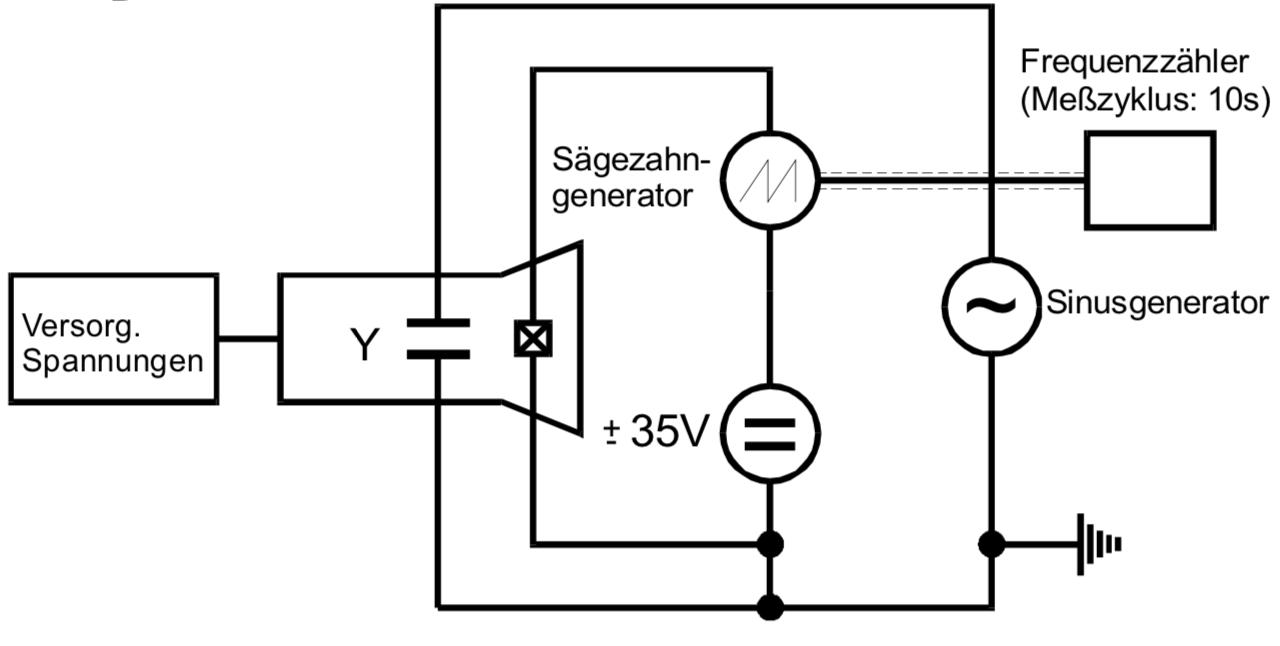
\includegraphics[width=10cm, height=5cm]{build/V501_b.png}
    \caption{Schaltbild eines Kathodenstrahl-Oszillographen. \cite{V501}}
    \label{fig:oszillograph}
\end{figure}

\subsection{Messung im Magnetfeld}
In diesem Versuchsteil sollen die spezifische Elektronenladung
und die Intensität des lokalen Erdmagnetfeldes bestimmt werden.

\subsubsection{Messung der spezifischen Elektronenladung}
Es soll die spezifische Elektronenladung bestimmt werden.
Dazu erzeugt ein Helmholtz-Spulenpaar ein annähernd homogenes
Magnetfeld. Dieses steht senkrecht zu dem Elektronenstrahl
einer Kathodenstrahlröhre.
Nach der korrekten Ausrichtung mithilfe eines speziellen
Kompasses wird bei konstanten
Beschleungigungsspannungen $U_B = \SI{250}{\volt}$ und 
$\SI{360}{\volt}$ die Verschiebung $D$ des Elektronenstrahls
in Abhängigkeit von den beiden Magnetfeldstärken gemessen. 
Dazu wird jeweils die
Stromstärke, die eingestellt werden muss, um den Leuchtfleck
auf die neun Linien des Koordinatennetzes zu bewegen,
abgelesen.

\subsubsection{Messung der Intensität des lokalen Erdmagnetfeldes}
Die Achse der Kathodenstrahlröhre wird in Nord-Süd-Richtung
des Erdmagnetfeldes ausgerichtet. Die Position des Leuchtflecks 
in dem Koordinatennetz wird erfasst.
Die Apparatur wird anschließend in Ost-West-Richtung ausgerichtet.
Der Leuchtfleck, dessen Position sich durch die Kraft des
Feldes geändert hat, wird durch Einschalten des Helmholtz-Feldes
wieder auf seine ursprüngliche Position bewegt, indem die Wirkung
des Erdmagnetfeldes durch den Spulenstrom $I_\text{hor}$ kompensiert
wird. Diese Stromstärke wird aufgenommen.
Anschließend wird mithilfe des speziellen Kompasses der Winkel
$\varphi$ zwischen der Horizontalebene und der Richtung des
Erdmagnetfeldes bestimmt.